\documentclass[10pt]{article}
\usepackage[pdftex]{graphicx}
\usepackage{subfig}
\usepackage{amsfonts}
\usepackage{amsmath}
\usepackage{calc}

% include other pdfs
\usepackage[final]{pdfpages}

% Shit I don't know.
\usepackage{enumerate}
\usepackage{amsmath}
\usepackage{ulem}

\usepackage{abstract}

% Fancy Headers and footers.
\usepackage{fancyhdr}

% For References.
\usepackage{natbib}

% This is for the page references.
% The TeX document must be built multiple times to work.
\usepackage{lastpage}

% This allows for multiple columns in one page.
\usepackage{multicol}


% This is for comments. (I think)
\usepackage{verbatim}

% This makes the references pretty.
\usepackage{hyperref}

\usepackage{indentfirst}

% This is for garbage.
\usepackage{lipsum}
\usepackage{abstract}

\def \TITLE {Tree Leaf Allometry}

%Math comp id: 13762
\def \GROUPID {13762}

% This makes the margins pretty with very little work.
\usepackage[margin=1in,lmargin=0.5in,rmargin=0.5in]{geometry}


\pagestyle{fancy}
\numberwithin{equation}{subsection}


\fancyhead{}
\fancyfoot{}

\fancyhead[CO,CE]{\TITLE}
\fancyfoot[CO,CE]{Mathematical Contest in Modeling}
\renewcommand{\footrulewidth}{0.4pt}


\lhead{\GROUPID}
%\rhead{Page \thepage\ of \pageref{LastPage}}
\rhead{\thepage}

\newlength{\imgwidth}

% This allows for block comments.
\newcommand{\ignore}[1]{}

\newcommand{\scalegraphics}[1]{%
    \settowidth{\imgwidth}{\includegraphics{#1}}%
    \setlength{\imgwidth}{\minof{\imgwidth}{\columnwidth}}%
    \includegraphics[width=\imgwidth,keepaspectratio]{#1}%
}

\begin{document}

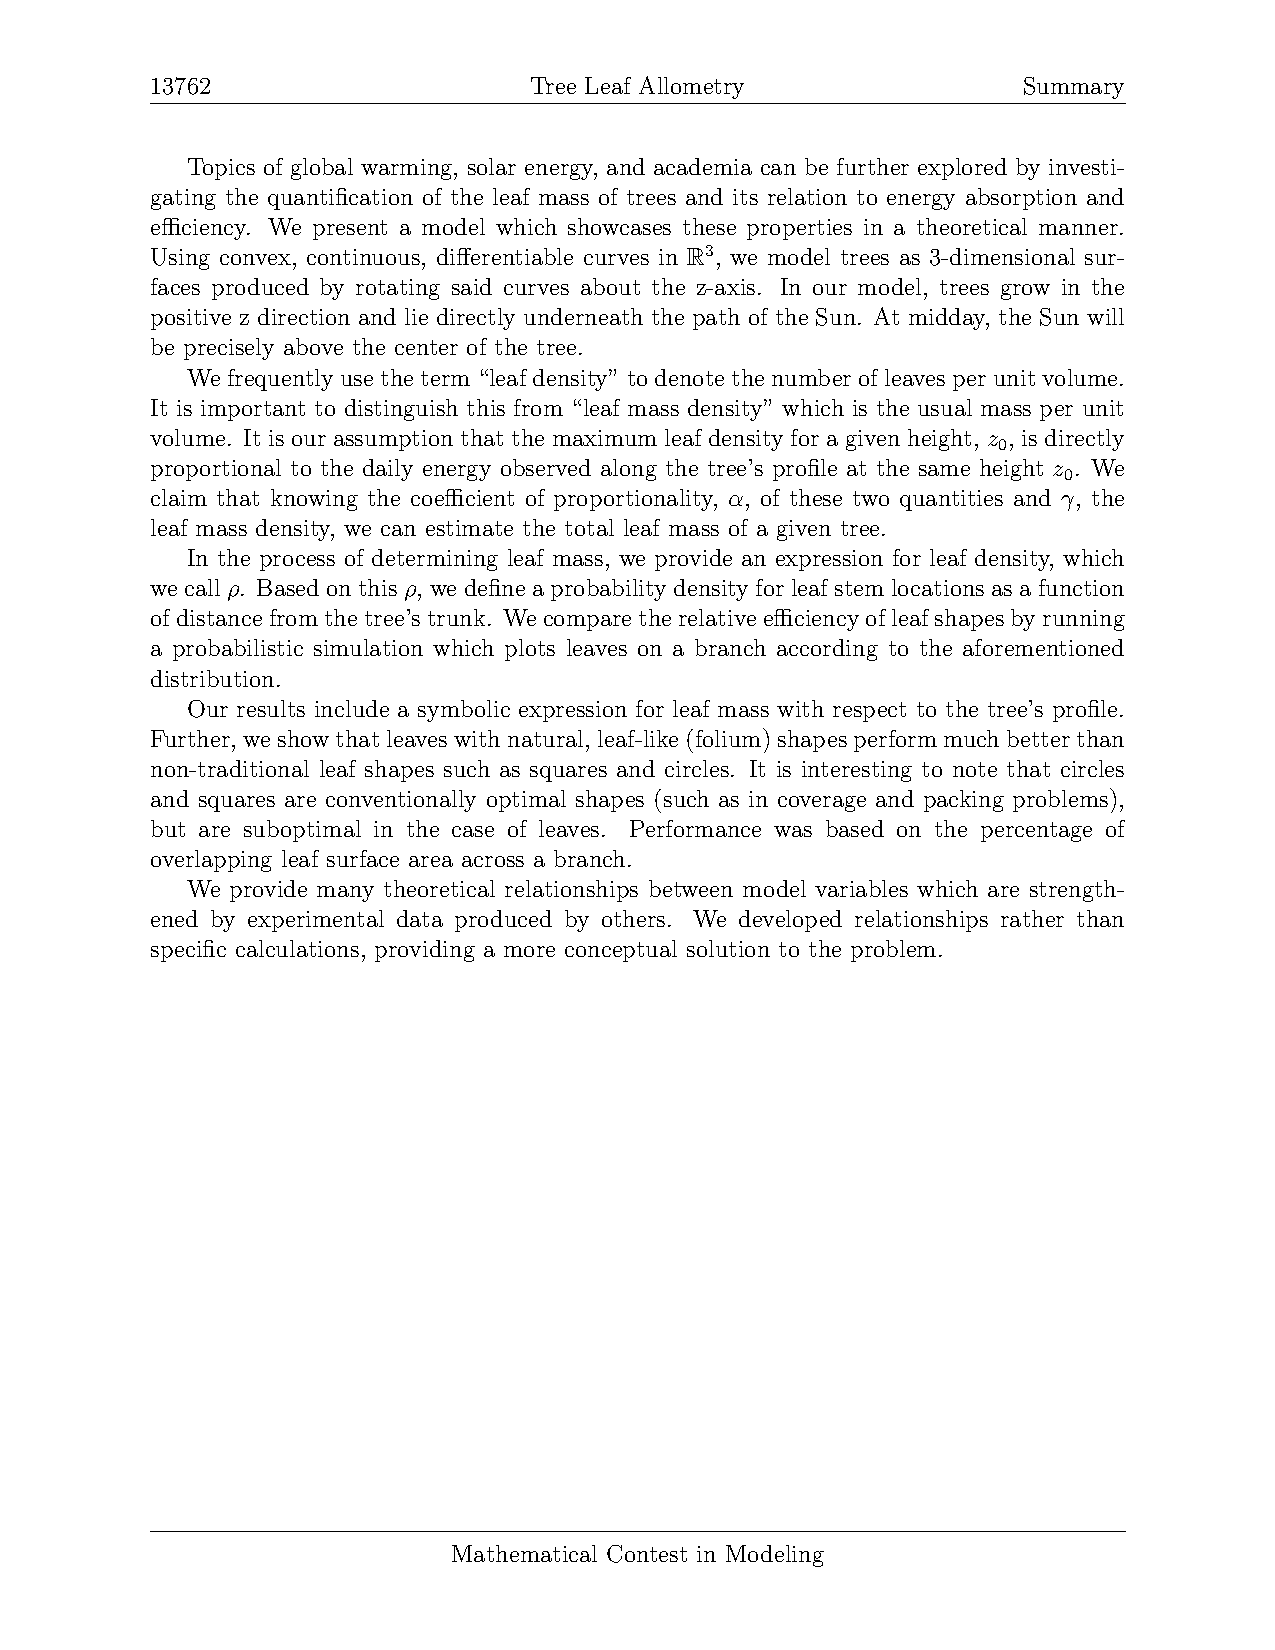
\includepdf{summary.pdf}
%\includepdf{letter.pdf}

\onecolumn
\title{\TITLE}
\author{Group \GROUPID}
\maketitle
\pagenumbering{gobble}
\begin{center}
\begin{minipage}{14cm}
\begin{abstract}
  
  
    We present a model for estimating tree allometry on leaf mass and leaf mass
    distributions for a given tree.  Certain more explicit formulations of the
    question such as which type of tree or which type of environment contain
    more or less leaf mass content are essentially trivial to answer and are
    briefly addressed.  We focus on the sun distribution of energy on the
    surface of the tree for a given day as the heart of our model.  We argue
    that the leaf mass distribution is strongly correlated to the energy
    distribution around the shell of the tree.  In addition, we compare surface
    area overlap of different leaf shapes distributed across a branch at
    arbitrary height.  The qualitative results of our model agree with that of
    trees found in southern Moravia. \citep{sunLeaf01}

\end{abstract}
\end{minipage}
\end{center}

\onecolumn

\pagenumbering{roman}

\tableofcontents
\listoffigures
\listoftables
\twocolumn
\pagenumbering{arabic}

\section{Introduction}

Modeling and quantifying leaf mass on an arbitrary tree has
applications in global warming, solar energy, and academia.  The
global warming applications are obvious, a greater/smaller leaf mass
implies greater/less carbon sequestration by photosynthesis producing
a warmer /cooler planet.  A less-obvious application is for design of
a solar panel and cell configurations based on leaf distributions to
allow for a more optimal scheme.  An even more abstract application is
the concept of looking at a conventional coverage problem as a
evolutionary programming problem.  We present a model based on sun
light collection on a convex tree shape for predicting growth density.
Using this model, we show how this density affects leaf overlap and
how a leaf shape reduces said overlap more effectively over
conventionally optimal shapes such as circles or squares.  These
results are directly applicable to other fields such as those
mentioned previously.


\subsection{Model Overview}
We model a tree as a rotated curve in $\mathbb{R}^3$ with the x-y axis
parallel to the Earth's surface and z being the direction in which the
tree grows. The Sun travels in an arc above the tree illuminating its
profile.

Throughout the paper, we use the term ``leaf density'' to denote the
number of leaves per unit volume. In most cases we talk about the leaf
density in relation to the lateral distance from the trunk. Note that
this is different than ``leaf mass-density'' which is the mass per
unit volume of a leaf.

We build a framework using both daily energy observed along the
profile of the tree, and leaf density to build a comprehensive model
for estimating the total leaf mass of the tree. Our model also allows
us to explore the efficiency of different leaf shapes.

\subsection{Assumptions}
\begin{enumerate}[$\bullet$]
    \item A tree's profile can be defined by a convex, continuous,
      differentiable curve rotated about the z axis. In other words,
      the tree is symmetrical around its trunk. While not a perfect
      fit for natural trees, it has been shown that most are
      symmetrical to some degree \citep{treeSymm01}.

    \item The intensity of light throughout the day is constant at
      approximately $580 \mathrm{W}/\mathrm{m}^2$, as a result of only
      $43\%$ of incident light being at a usable
      wavelength\citep{plantAbsrb01}. Considered trees lie directly
      underneath the Sun's path through the sky.

    \item Horizontal leaf density follows a logistic curve which
      increases with distance from the trunk.  Logistic curves occur
      frequently in nature, and this type of distribution has been
      seen in tree growth patterns \citep{sigmoid01},
      \citep{sigmoid02}.

    \item Maximum leaf density at a given height is proportional
      to the daily energy observed along the profile at that height.
      This is a natural assumption which loosely means that trees will
      grow more leaves where more sunlight is present. This behavior
      is also noted in \citep{sunLeaf01}.

    \item Leaf mass-density, $\gamma$, is constant across all leaves
      on a tree \citep{massdensity01}.
\end{enumerate}

\subsection{Problem Definition}
Suppose $x = l(z)$ is a convex, continuous, and differentiable curve
which when rotated about the z axis gives the surface of a tree. Using
only $\gamma$, the mass-density of leaves, and $\alpha$, the
proportionality constant between the daily energy and maximum leaf
density at a given height, determine the leaf mass of the tree. Also
discuss the efficiency of leaf shape in terms of overlapping area.

\section{Model and Methods}

We model a tree by taking some function $x = l(z)$ and rotating it
about the $z$ axis. The resulting three-dimensional surface is the
profile of some tree $L$. We require $l(z)$ to be convex, continuous,
and differentiable for $z_0 \le z \le z_1$ where $z_0$ and $z_1$ are
the lower and upper bounds for the tree. \\

\begin{figure}[h!]
  \caption{Hypothetical Tree: $l(z)=\sqrt{1-(\frac{z}{2})^2}$}
  \centering
  \scalegraphics{img/lz.png}
  \label{fig:l(z)}
\end{figure}

For example,  take $l(z) = \sqrt{1-(\frac{z}{2})^2}$, rotate it around
the z axis giving a surface which represents the profile of a tree
(see {\bf Figures~\ref{fig:l(z)} and~\ref{fig:L}}). Describing tree
profiles in this fashion is not only convenient, but fairly
representative of trees in nature \citep{treeSymm01}. 

\begin{figure}[h!]
  \centering
  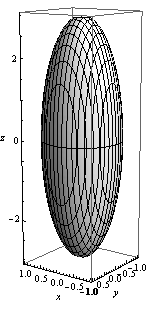
\includegraphics[width=120px]{img/L.png}
  \caption{Tree Surface $L$}
  \label{fig:L}
\end{figure}

Having a model of trees in $\mathbb{R}^3$, we now wish to represent
incoming sunlight in relation to our tree $L$. To simplify this
relationship, we assume the Sun's path coincides with $y=0$; in other
words, the Sun travels directly over the tree along the $x$ axis. We
set the x-y plane parallel to the Earth's surface, and let $\theta_t$
denote the angle rays from the Sun make with the positive $x$ axis at
time $t$. Letting $t$ range from $0$ to $1$ we have $\theta_t =
\theta_{min} + t(\theta_{max} - \theta_{min})$ where $\theta_{min}$
and $\theta_{max}$ are the minimum and maximum angles for which Sun
rays will reach $L$ respectively.

We let $\vec{T_z}$ denote the tangent vector at a point \\ $P$ =
($l(z)$, 0, $z$) on $L$. The intensity vector $\vec{I_\theta}$
represents a Sun ray that makes an angle $\theta$ with the x-y
plane. $|\vec{I_\theta}| = 580$ for all $\theta$
\citep{sunLight02}. {\bf Figure~\ref{fig:vectors}} shows the
previously defined vectors and angles.


\begin{figure}[h!]
  \centering
  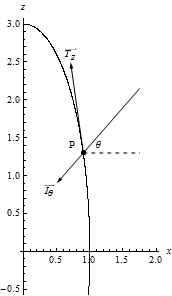
\includegraphics[width=120px]{img/vectors.png}
  \caption{Angles and vectors on $l(z)$}
  \label{fig:vectors}
\end{figure}


\subsection{Daily Energy Along the Tree Profile}
We now wish to determine the total energy a point receives over one
period (a full day). First, we examine the instantaneous intensity at
point $P$ = ($l(z)$, 0, $z$) using \citep{website:sunLight01}:
\begin{center}
  \begin{equation}\label{eqn:intbasic}
    |I_z| = |I_\theta| \  \cos\phi
  \end{equation}
\end{center}

Here, $\phi$ is the angle between $\vec{I_\theta}^{\perp}$ and
$\vec{T_z}$, notice this is just the projection of $\vec{I_\theta}$ on
to $\vec{T_z}$ as seen in {\bf Figure ~\ref{fig:vectors}}. Solving for $\phi$ using the definition of the dot
product yields:

\begin{center}
  \begin{gather}
    \phi = \cos^{-1} \left(\dfrac{\vec{I_0}^{\perp} \cdot \vec{T_z}}{|\vec{I_0}^{\perp}| |\vec{T_z}|}\right) \nonumber \\
    I(z,\theta) = |I_\theta|\left(\dfrac{-\sin\theta \  l'(z) + \cos\theta}{\sqrt{1+(l'(z))^2}}\right)\label{eqn:intpoint}
  \end{gather}
\end{center}

Equation~\eqref{eqn:intpoint} defines the instantaneous intensity at a
point ($l(z)$, 0, $z$) for a given $\theta$. Having an expression for
intensity allows us to determine the total energy a point receives
over the course of one full day. To calculate total energy, we must
integrate intensity over a full period, $0 \le t \le 1$ \citep{sunPower01}.

\begin{center}
  \begin{equation}
    \begin{split}
      E(z) &= \int_0^1 I(z,\theta_t) \mathrm{d}t \\
      &= \int_0^1 |I_\theta|\left(\dfrac{-\sin\theta \  l'(z) + \cos\theta}{\sqrt{1+(l'(z))^2}}\right) \mathrm{d}t
    \end{split}
  \end{equation}
\end{center}

Continuing with our example of a tree with profile $l(z) =
\sqrt{1-(\frac{z}{2})^2}$, we graph the energy observed per day for
each z for which our tree is defined ($-3 \le z \le 3$). This graph
({\bf Figure~\ref{fig:energy}}) shows exactly what you might expect:
very small energy at the base of the tree, fairly average energy in
the middle, and very high energy near the top.


\begin{figure}[h!]
  \centering
  \scalegraphics{img/energy.png}
  \caption{Energy over a full day with respect to z}
  \label{fig:energy}
\end{figure}


\subsection{Estimating Leaf Mass}

Our approach to estimating the leaf mass requires knowledge of the
leaf density, $\rho$, as a function of height and lateral distance
from the trunk. It is our assumption that the tree is fully
symmetrical about the $z$ axis, thus we simply work in the cross
section at $y=0$.

We believe that the leaf density is logistic with respect to x, the
lateral distance from the trunk. For small x near the trunk, there
will be few leaves, but approaching the boundary of the tree profile,
the leaf density must grow rapidly. Not only is this an intuitive
model, but is mentioned in \citep{sigmoid02}. We suppose that the leaf
density function is of the approximate form ({\bf
  Figure~\ref{fig:rho}}) with $\rho_{\mathrm{max}}(z)$ being the maximum leaf
density for a given height:

\begin{center}
  \begin{equation}
    \rho(z,x) = \dfrac{\rho_{\mathrm{max}}(z)}{1+e^{-6(\frac{2x}{l(z)}-1)}} \label{eqn:rho}
  \end{equation}
\end{center}


\begin{figure}[h!]
  \centering
  \scalegraphics{img/rho.png}
  \caption{Shape of $\rho(z,x)$ for fixed $z$}
  \label{fig:rho}
\end{figure}


Integrating equation~\eqref{eqn:rho} across all values of z and then
going around the $z$ axis with $\theta$ going from 0 to $2\pi$, we
find the leaf mass proprotional to the following expression:

\begin{center}
  \begin{equation}
    \begin{split}
      m &= \int_0^{2\pi} \int_0^{h} \int_0^{l(z)} \gamma \rho(z,x) \ \mathrm{d}x \mathrm{d}z \mathrm{d}\theta \\
      &= 2\pi\gamma \int_0^{h} \left(\int_0^{l(z)} \dfrac{\rho_{\mathrm{max}}(z)}{1+e^{-6(\frac{2x}{l(z)}-1)}} \mathrm{d}x\right) \mathrm{d}z \\
      &= 2\pi\gamma \int_0^{h} \rho_{\mathrm{max}}(z) \left[ \frac{l(z)}{12} log\left( e^{\frac{12x}{l(z)}} + e^6 \right) \right]_0^{l(z)} \mathrm{d}z
    \end{split}
  \end{equation}
\end{center}

We have now defined a leaf mass function which depends on the
parameters:

\begin{enumerate}
\item $l(z)$ The profile function of a tree.
\item $\rho_{\mathrm{max}}(z)$ The maximum leaf density at a height $z$.
\item $h$ The height of the tree.
\item $\gamma$ The leaf mass-density of the tree.
\end{enumerate}


\subsection{Relationship Between Maximum Leaf \\Density and Energy}
Our final discussion brings together our expression for the leaf
density with energy. We do this by noting that since it has been shown
that in certain cases the maximum leaf density at a given height is
directly proportional to the daily energy observed at that point
\citep{sunLeaf01}. Using notation described thus far, we make the
claim that $\rho_{\mathrm{max}}(z) \propto E(z)$.

Using this relationship, we now rewrite our expression for the leaf
mass using the substitution $\alpha E(z) = \rho_{\mathrm{max}}(z)$. We start by rewriting
equation~\eqref{eqn:rho} as:

\begin{center}
  \begin{equation}
    \begin{split}
      \rho(z,x) &= \dfrac{\rho_{\mathrm{max}}(z)}{1+e^{-6(\frac{2x}{l(z)}-1)}} \\
      &= \dfrac{\alpha E(z)}{1+e^{-6(\frac{2x}{l(z)}-1)}}
    \end{split}
  \end{equation}
\end{center}

Finally, bringing everything together, we find an expression for the
leaf mass of a tree using the new version of $\rho(z,x)$. This
equation is exciting because it lets us approximate the leaf mass of a
tree needing knowledge only of $l(z)$ and $\alpha$, the
proportionality constant for $\rho_{\mathrm{max}}(z)$ and $E(z)$.

%\begin{minipage}[l]{\linewidth}
\begin{center}
  \begin{equation}
    \begin{split}
      m &= 2\pi\alpha \int_0^{h}
      E(z) \left[ \frac{l(z)}{12} log\left( e^{\frac{12x}{l(z)}} + e^6 \right) \right]_0^{l(z)} \mathrm{d}z \\
      &= 2\pi\alpha \int_0^{h}
      \left[\int_0^1 I(z,\theta_{t})dt\right]
      \left[ \frac{l(z)}{12} log\left( e^{\frac{12x}{l(z)}} + e^6 \right) \right]_0^{l(z)} \mathrm{d}z \\
      &= 2\pi\alpha |I_\theta| \int_0^{h}
      \bigg(\int_0^1 \dfrac{-\sin\theta_t \  l'(z) + \cos\theta_t}{\sqrt{1+(l'(z))^2}} dt \\
      & \;\;\;\;\;\;\;\;\;\;\;\;\;\;\;\;\;\;\;\;\;\;\;\;\;\;\;\;\;\;\left[ \frac{l(z)}{12} log\left( e^{\frac{12x}{l(z)}} + e^6 \right) \right]_0^{l(z)} \bigg) \mathrm{d}z \\
      %&= 2\pi\alpha |I_\theta| \int_0^{h} \bigg(\int_0^1 \dfrac{-\sin\theta_t \  l'(z) + \cos\theta_t}{\sqrt{1+(l'(z))^2}} dt \\
      %& \;\;\;\;\;\;\;\;\;\;\;\;\;\;\;\;\;\;\;\;\;\;\;\;\;\;\;\;\;\;\left(l(z)\log(\frac{e^{1}) + e^{6}}{1 + e^{6}} \right) \bigg) \mathrm{d}z
    \end{split}
  \end{equation}
\end{center}

  
\subsection{Leaf Shape Overlap Comparison}

We now explore the relationship between a leaf's shape and the ratio
of overlapping surface area of leaves on a branch at a given height on
a tree. To do this, we model a branch as a horizontal line in the x-y
plane at some fixed $z_0$. Supposing there are $n$ leaves on this
branch, we would expect them to be distributed across the branch
according to a distribution based on $\rho(z_0,x)$.

Appealing to probability theory, we need to express this distribution
as a probability density function. Using equation~\eqref{eqn:rho}, we
define the following function $f$ as a PDF describing the distribution
of stem locations on the branch at height $z_0$. Note that $f(x) = 0$
for $x < 0$ and $x > l(z)$.

\begin{center}
  \begin{gather}
    \rho_{\mathrm{mass}} = \int_0^{l(z_0)}\rho(z_0,x)\mathrm{d}x \nonumber \\ 
    f(x) = \dfrac{\rho(z_0,x)}{\rho_{\mathrm{mass}}} \label{eqn:fx}
  \end{gather}
\end{center}

Next, we determine the percentage of overlapping area on this $z_0$
branch with leaves of three different shapes: circle, square, and folium
(which we describe shortly). Fixing the area of each leaf to 1
$\mathrm{cm}^2$, we place $n$ leaves along the $x$ axis according to
the distribution $f$~\eqref{eqn:fx}.

To determine the location of the stems, we use inverse transformation
sampling to choose values of $x$ according to distribution
$f$. Essentially, we evaluate the inverse cumulative distribution of
$f$ at uniformly random values between 0 and 1. This method is
outlined in \citep{invsample01}. We calculate the CDF as:

\begin{center}
  \begin{equation}
    \begin{split}
      F(y) &= \int_0^y f(x)\mathrm{d}x \\
      &= \frac{1}{\rho_{\mathrm{mass}}}\int_0^y \rho(z_0,x) \mathrm{d}x
    \end{split}
  \end{equation}
\end{center}

At this point, keeping track of an analytic function had become
unwieldly. We need the inverse of $F$ which we will be using to sample
$x$ values at our $z_0$. Using MATLAB's built-in interpolation
functionality, we were able to approximate $F^{-1}$ to a high degree
of accuracy.

\subsubsection{Quick Discussion About Shapes}
Before we continue, we would like to mention our justification of the
shapes we analyzed. First, the folium shape which literally means
``leaf'' or ``petal''. We believe it to be a good representation of an
average leaf, see {\bf Figure~\ref{fig:folium_shape}}. Unfortunately,
we were constrained to convex shapes due to the geometry libraries we
had available. Circles and squares seem to be good candidates for
convex shapes at other ends of the spectrum.

\begin{figure}[h!]
  \centering
  \scalegraphics{img/folium_single.png}
  \caption{Folium shape described by:\\ $r=-\mathrm{b}\cos\theta +
    4\mathrm{a}\cos\theta \sin2\theta$ ~\citep{foliumshape01}}
  \label{fig:folium_shape}
\end{figure}


\section{Results and Discussion}
We started with a very basic model of a tree and have developed
sophisticated solutions to energy, mass, and shape considerations. As
a summary of our results, we list a few key equations:

\begin{center}
  \begin{equation*}
    E(z) = \int_0^1 |I_\theta|\left(\dfrac{-\sin\theta \  l'(z) + \cos\theta}{\sqrt{1+(l'(z))^2}}\right) \mathrm{d}t
  \end{equation*}
  \begin{equation*}
    \rho(z,x) = \dfrac{\alpha E(z)}{1+e^{-6(\frac{2x}{l(z)}-1)}} 
  \end{equation*}
  \begin{equation*}
    m = 2\pi\alpha \int_0^{h}
      E(z) \left[ \frac{l(z)}{12} log\left( e^{\frac{12x}{l(z)}} + e^6 \right) \right]_0^{l(z)} \mathrm{d}z
  \end{equation*}
\end{center}

Based on these relationships we were able to set up a very detailed
simulation modeling the effect leaf shapes have on surface area
efficiency. Using MATLAB, and the MPT library \citep{mpt} we
represented individual leaves as convex polytopes. Using the inverse
cumulative distribution for sampling lateral distances (as discussed
above) we were able to plot a series of leaves across an imaginary
branch at any given height. Leaves were distributed according to
$\rho(z,x)$, the leaf density giving an accurate picture of a typical
branch.

We used the same distances for each leaf shape as to provide a
foundation for fairly judging performance. Upon calculating the
distances, we placed a leaf at each point and the calculated the
overlapping surface area. Our measure was the average percent of area
overlapped for each leaf. {\bf Figure~\ref{fig:shapes}} shows the plot
created for each shape. Green outlines indicate a leaf, and red filled
area represents overlapping area.

{\bf Table~\ref{tab:overlap}} shows the average overlap for each leaf
shape as well as the parameters to the simulation. There is quite a
large disparity between the folium shape and the two non-traditional
leaf shapes. As we would expect, the natural, leaf-like shapes perform
much better.

\subsection{Further Research}
For a closer examination of leaf mass with respect to tree profile, we
would suggest investigating different $l(z)$ curves. Throughout this
paper, we use a simple ellipsoid tree profile as our key example, but
there are many other natural tree shapes.

During our research, we did not uncover any experimental data that
shed light on the relationship between tree profile and leaf mass. It
would be revealing to pit our model's prediction against hard data. 

Finally, it would be interesting to extend our model of light
intensity from the Sun to include attenuation as the radiation travels
through the atmosphere. 


\begin{table}[h!]
    \begin{tabular}{|l|l|l|l|l|}
        \hline
        Leaf Shape & Branch Length & Leaves & Leaf Size & $\%$ Overlap \\ \hline
        Folium    & $40$cm & 30 & $1 \mathrm{cm}^2$  & $61.446\%$    \\ \hline
        Square & $40$cm & 30 & $1 \mathrm{cm}^2$  & $75.805\%$    \\ \hline
        Circular & $40$cm & 30 & $1 \mathrm{cm}^2$  & $69.460\%$    \\ \hline
        Folium & 60cm & 30 & $1 \mathrm{cm}^2$ & $46.678\%$ \\ \hline
        Square & 60cm & 30 & $1 \mathrm{cm}^2$ & $56.677\%$ \\ \hline
        Circular & 60cm & 30 & $1 \mathrm{cm}^2$ & $54.628\%$ \\ \hline
    \end{tabular}
    \caption{Overlap comparison for circle, square and folium shaped leaves.}
    \label{tab:overlap}
\end{table}

\begin{figure}[h!]
  \centering
  \scalegraphics{img/shapes.png}
  \caption{Branch visualization for each leaf shape.}
  \label{fig:shapes}
\end{figure}

\section{Conclusion}
We have built a powerful yet comprehensible framework modeling many
properties of a tree based on a few important characteristics. Given
height, profile, and $\alpha$ as defined above, we can calculate:

\begin{enumerate}
\item Total leaf mass.
\item Leaf density.
\item Estimate for total number of leaves.
\item Estimate maximum energy absorbed per day.
\end{enumerate}

By keeping our model generic, we retained the ability to keep separate
the notions of a tree profile and a leaf shape. We can extend our
model to encompass most any tree that fits within our simple
assumptions. Finally, an encouraging result of our model is that
leaves of a natural folium shape are more efficient in terms of
overlapping surface area.


\onecolumn
\bibliography{references}
\bibliographystyle{plainnat}
\nocite{*}
\addcontentsline{toc}{section}{References}


\end{document}
